\documentclass[a4paper,11pt]{report}

\usepackage{amsmath}
\usepackage{fullpage}
\usepackage{tikz}

\usetikzlibrary{graphs,graphs.standard}

\makeatletter
\pgfmathdeclarefunction{alpha}{1}{%
  \pgfmathint@{#1}%
  \edef\pgfmathresult{\pgffor@alpha{\pgfmathresult}}%
}

\author{Sylvain Julmy}
\date{\today}

\setlength{\parindent}{0pt}

\begin{document}

\begin{center}
  \Large{
    Mathematical Methods for Computer Science 1\
    Fall 2017
  }
  \noindent\makebox[\linewidth]{\rule{\linewidth}{0.4pt}}

  Series 4
  \vspace*{1.4cm}

  Sylvain Julmy
  
  \noindent\makebox[\linewidth]{\rule{\linewidth}{0.4pt}}
\end{center}

\section*{\texttt{1}}
\subsection*{a)}
To show that the graph $G = (V = \{\text{ all two-element subsests of }\{1,2,3,4,5\}\},
E =\{\{A,B\} | A \cap B= \emptyset \}\})$, we could use the following bijection:
\begin{align*}
  f : \{ f &\mapsto \{1,2\}, \\
         j &\mapsto \{2,4\}, \\
         i &\mapsto \{3,4\}, \\
         h &\mapsto \{3,5\}, \\
         g &\mapsto \{1,5\}, \\
         a &\mapsto \{4,5\}, \\
         b &\mapsto \{2,3\}, \\
         c &\mapsto \{1,4\}, \\
         d &\mapsto \{2,5\}, \\
         e &\mapsto \{1,3\}\}
\end{align*}

With the following graph

\begin{center}
\begin{tikzpicture}[every node/.style={draw,circle,very thick}]
  \graph [clockwise,math nodes] {
    subgraph C_n [V={a,b,c,d,e},name=A, radius=2cm]; 
    subgraph I_n [V={f,g,h,i,j},name=B, radius=1cm];
    \foreach \x [evaluate={%
        \i=alpha(\x);
        \j=alpha(mod(\x+1,5)+6); 
        \k=alpha(\x+5);}] in {1,...,5}{
      A \i -- B \k;
      B \j -- B \k;
    }
  }; 
\end{tikzpicture}    
\end{center}

We ca see that the intersection of the sets of two adjacents nodes are empty.

\subsection*{b)}

The following graph

\begin{center}
\begin{tikzpicture}[every node/.style={draw,circle,very thick}]
  \graph [clockwise,math nodes] {
    subgraph C_n [V={a,b,c,d,e},name=A, radius=2cm]; 
    subgraph C_n [V={f,g,h,i,j},name=B, radius=1cm];
    \foreach \x [evaluate={%
      \i = alpha(\x);
      \k = alpha(\x+5);}] in {1,...,5}{
      A \i -- B \k;
    }
  };
\end{tikzpicture}    
\end{center}

is not isomorphic to the petersen graph, because this graph has an Hamiltonian
cycle and the Petersen graph does not, so this graph is Hamiltonian and the
Petersen graph is not Hamiltonian.

\section*{\texttt{2}}

\subsection*{a)}

In a graph with $n$ vertices, if a vertice $v$ has a degree $n-1$, it means that he
is connected to every other vertices of the graph except itself. It implies that
from any vertices other than $v$, we can go to $v$ and then to an another
vertice of the graph, so every vertices is accessible from any other vertices
with $2$ jump. Therefore, the graph is connected.

\subsection*{b)}

We imagine we separate the graph G into two group of 7 vertices each. In each
groupe we fully connected the nodes so every nodes of the two groups has a
degree $6$ :

\begin{minipage}{0.49\textwidth}
  \begin{center}
    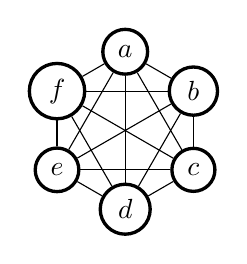
\begin{tikzpicture}[every node/.style={draw,circle,very thick}]
      \graph [clockwise,math nodes] {
        subgraph K_n [V={a,b,c,d,e,f},name=A, radius=1cm]; 
      };
    \end{tikzpicture}
  \end{center}
  \end{minipage}
  \begin{minipage}{0.49\textwidth}
  \begin{center}
    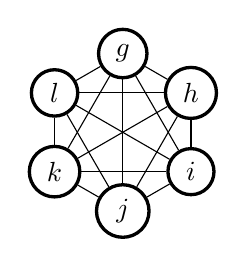
\begin{tikzpicture}[every node/.style={draw,circle,very thick}]
      \graph [clockwise,math nodes] {
        subgraph K_n [V={g,h,i,j,k,l},name=B, radius=1cm];
      };
    \end{tikzpicture}
  \end{center}
\end{minipage}

In order to have a $7$-regular graph, we have to connect every node of each
graph to an another ones that is not part of the opposing graph. Due to $7 + 7 =
14$, we have just $1$ node left to connect each nodes of each subgraph. So, each
vertices of each subgraph is connected to the one left, so the graph is
connected according to the previous point in exercice $2$.

\section*{\texttt{3}}
\subsection*{a)}

From the two following degrees sequences : $A = (5,4,3,2,2,1)$ and $B =
(5,4,3,2,1,1)$, only $B$ could be a degree sequences in a graph with $6$
vertices because $5+4+3+2+1+1 = 16$ is even and $5+4+3+2+2+1 = 17$ is odd, and
the sum of all the degrees of a Graph is even.

\subsection*{b)}

No, we represent the segment as vertices in a graph $G$ and the intersections as
connections between two vertices. So if a segment $s_1$ intersect with a segment
$s_2$, $s_1$ and $s_2$ are adjacent in $G$.

We know that the segments set we want to draw is $3$-regular, so there is $9$
vertices with a degree $3$ for each, then the sum of all the degrees is :
$\sum_{i=1}^9 3 = 3*9 = 27$, $27$ is odd so it is not possible because the sum
of the degree of all vertices in a graph is even.

\section*{\texttt{4}}

\subsection*{a)}

We take the smallest adjacency matrix $A_G$ that could contains a triangle :
\[
\begin{pmatrix}
0 & a_{12} & a_{13} \\
a_{21} & 0 & a_{23} \\
a_{31} & a_{32} & 0
\end{pmatrix}
\]

If $A_G$ contains a triangle, it means that we have a fully connected adjacency
matrix :

\[
\begin{pmatrix}
0 & 1 & 1 \\
1 & 0 & 1 \\
1 & 1 & 0
\end{pmatrix}
\]

If $A_G^3$ contains a $0$ in his diagonals, it means that there would be a $0$
in a row and in a columns (because the matrix diagonals is a mirror, if $a$ is
connected to $b$, then $b$ is connected to $h$) which result in a $0$ in the
diagonals of $A_G^3$. Example with a triangle:
\[
\begin{pmatrix}
0 & 1 & 1 \\
1 & 0 & 1 \\
1 & 1 & 0
\end{pmatrix}^3 =
\begin{pmatrix}
2 & 3 & 3 \\
3 & 2 & 3 \\
3 & 3 & 2
\end{pmatrix}
\]

And without a triangle

\[
\begin{pmatrix}
0 & 0 & 1 \\
0 & 0 & 1 \\
1 & 1 & 0
\end{pmatrix}^3 =
\begin{pmatrix}
0 & 0 & 2 \\
0 & 0 & 2 \\
2 & 2 & 0
\end{pmatrix}
\]

Because $a_{12}$ and $a_{21}$ are $0$, $a_{22}$ would be $0$ anyway after
multiple power of the matrix.

We have show this for a graph of $3$ vertices, but we can extends it to any
graph, because a triangle in any graph is a subgraph which has $3$ vertices and
his fully connected.

\subsection*{b)}

In a graph, a triangle is a walks of length $3$, by using the matrix adjacency
$A_G$, the number of walks between vertex $i$ and $j$ of length $n$ is given by
the element $(i,j)$ of the matrix $A_G^n$. Because a triangle is a walks of
length $3$, we compute the trace of $A_G^3$, which gives the total number of
triangle in $G$. But, we have to divide $trace(A_G^3)$ by $6$, because the
adjacency matrix is symetric and because a triangle has $3$ vertices, we counted
a walks $3$ times for $3$ vertices. Then, we have the number of triangle in $G$
is given by
\[
  trace(A_G^3) \frac{1}{\underbrace{3}_{\text{a triangle has $3$ vertices}} \underbrace{2}_{\text{$A_G$ is symetric}}}
\]

\section*{\texttt{5}}

\subsection*{a)}

The is $\frac{n!}{2n}$ distinct Hamiltonian cycle in the complete graph $K_n$.
From any vertices of the graph, we can choose $n-1$ different path, then $n-2$,
hand so on... so we have $(n-1)!$ differents cycle, we divide by $2n$ because the
cycle $(1,2,3,4)$ is the same as the cycle $(4,1,2,3)$ and $(3,4,1,2)$, hand so
on. Therefore we have $\frac{(n-1)!}{2} = \frac{n!}{2n}$.

\subsection*{b)}

In any graph $P_{m,n}$, there is always a Hamiltonian path that simply traverse
the rows in alternate direction, if $m$ is even (or $n$, we could juste
transpose the grid graph to inverse $m$ and $n$), so there would be a path to
come back to the start of the cycle.

The idea is to start from the top left and traverse the first row, and the
second except for the first element of the second row, the we go to the third
and so on. In order to go and comeback, we need to have $2$ row, so an even
number of row gives us the go and comeback strategy.

\subsection*{c)}

If $n$ and $m$ are odd, it means that we can't comeback after the ``go'' from
the previous exercice.

\end{document}